\documentclass[conference]{IEEEtran}
\IEEEoverridecommandlockouts

\usepackage{cite}
\usepackage{amsmath,amssymb,amsfonts}
\usepackage{graphicx}
\usepackage{booktabs}
\usepackage{textcomp}
\usepackage{xcolor}
\usepackage{url}
\usepackage{hyperref}

\hypersetup{colorlinks=true, linkcolor=black, citecolor=black, urlcolor=blue}

\begin{document}

\title{Automated Stylistic Anomaly Detection in\\
Artwork Collections Using Deep Learning}

\author{
\IEEEauthorblockN{Yeva Stepanyan}
\IEEEauthorblockA{Akian College of Science and Engineering\\
American University of Armenia\\
Yerevan, Armenia\\
yeva\_stepanyan@edu.aua.am}
\and
\IEEEauthorblockN{Gurgen Hovakimyan (Supervisor)}
\IEEEauthorblockA{Akian College of Science and Engineering\\
American University of Armenia\\
Yerevan, Armenia\\
ghovakimyan@aua.am} }

\maketitle

\begin{abstract}
Identifying paintings that stylistically deviate from a genre collection has traditionally required art-historical expertise and is difficult to scale to digital archives containing hundreds of thousands of works. This paper treats stylistic anomaly detection as an unsupervised problem over deep visual embeddings and compares four pretrained representations (ResNet-50 in single-layer and multi-layer configurations, DINOv2 ViT-B/14, and VGG-19 Gram matrices) combined with eleven detection algorithms covering distance, density, isolation, reconstruction, distributional, and clustering paradigms. Experiments are conducted on a curated WikiArt subset of 7{,}500 paintings drawn from five canonical genres, each contaminated by a controlled five-percent injection of paintings from either stylistically distant or stylistically adjacent genres. The strongest combination, multi-layer ResNet-50 with a deep autoencoder on raw embeddings, reaches a mean AUC-ROC of 0.95 across genres under standard injection and 0.92 under adjacent-genre injection. A second finding is that the ranking of the best detectors flips between semantic-content embeddings and style-texture embeddings. A qualitative review by an art historian shows that detection performance tracks art-historical assessments of within-genre coherence and surfaces concrete limitations regarding genre granularity, medium mismatch, and the difference between statistical and canonical norms. The framework is intended as a decision-support tool for large-scale collection analysis.
\end{abstract}

\begin{IEEEkeywords}
anomaly detection, deep representation learning, art history, unsupervised learning, computer vision, WikiArt
\end{IEEEkeywords}

\section{Introduction}
\label{sec:introduction}

The digitization of art collections has created archives far too large to review by hand. Museums, galleries, and crowd-sourced projects such as WikiArt now host hundreds of thousands of works organized by attributed style, genre, and period. Within these archives, deciding which paintings truly represent a movement and which deviate from it still depends entirely on human experts. These judgments are important because they shape attribution debates, exhibition planning, provenance research, conservation work, and the way art is taught and studied. However, relying entirely on expert review does not scale well to collections of this size. Stylistic classification can vary even between specialists, and museums rarely have the time or resources to examine every work in detail.

The challenge is in how the style is represented. Style cannot be defined as a simple label that is assigned directly. It emerges from patterns in visual features and they can vary consistently between different artistic movements. A painting can differ from others in brushwork, palette, composition, or subject matter. Any of those differences might be a genuine stylistic deviation signal or just noise. Identifying which paintings belong to a movement, and which do not, requires learning what the style of that movement looks like from within, rather than drawing a line between two fixed categories.

Prior work has mainly focused either on supervised style classification \cite{lecoutre, sandoval, agarwal, karayev} or on physical anomaly detection in cultural heritage images
\cite{mezina, pu, ji}. Neither directly addresses stylistic anomaly
detection in photographed paintings.

This paper addresses that gap. Given a collection of paintings nominally belonging to a genre, can deep learning identify the works that stylistically do not fit? Three research questions guide the study:

\begin{itemize}
\item \textbf{RQ1.} Which combination of deep visual embedding and
unsupervised detection algorithm most reliably identifies stylistic outliers in a painting collection?
\item \textbf{RQ2.} How does dimensionality reduction, specifically
PCA to fifty components, affect detection performance, and does this effect vary across embedding families?
\item \textbf{RQ3.} Which visual regions of an anomalous painting
carry the anomaly signal, and to what extent do these regions align with art-historical interpretation?
\end{itemize}

There are three main contributions that this work provides. First, it systematically compares $4 \times 11 = 44$ embedding and method combinations across five canonical genres and two injection difficulties, producing 440 AUC-ROC measurements that cover the full design space. Second, it finds and explains a consistent ranking inversion: the detectors that work best on semantic embeddings (ResNet, DINOv2) are not the same as those that work best on style-texture embeddings (VGG-19 Gram matrices), which means stylistic anomaly detection is a complex problem consisting of several aspects, each requiring a different approach. Third, it includes an expert art-historian review with concrete visual examples that connect the technical findings to art-historical interpretation.

The remainder of the paper is organized as follows. Section~\ref{sec:related_work} reviews prior work on computational analysis of artistic style and on unsupervised anomaly detection in cultural heritage. Section~\ref{sec:methodology} describes the experimental framework, including dataset construction, controlled anomaly injection, embedding extraction, and the detection algorithms. Section~\ref{sec:results} presents the quantitative findings. Section~\ref{sec:analysis} provides an interpretative analysis of detector behavior, ranking-inversion effects, per-genre differences, and the expert review. Section~\ref{sec:discussion_limitation} discusses the limitations of the framework and the conditions under which it is appropriate. Section~\ref{sec:conclusion} answers each research question, states the main scientific contributions, and outlines future work.

\section{Related Work}
\label{sec:related_work}

\subsection{Supervised classification of artistic style}

Computational analysis of artistic style predates deep learning, with earlier work drawing on image statistics, formal-feature analysis, and metric-learning approaches to study paintings quantitatively \cite{graham, wasielewski}. The earliest and still most common approach in computational art analysis treats style as a classification problem. Karayev et al.~\cite{karayev} show that mid-level features extracted from networks pretrained on natural images carry enough stylistic signal to discriminate among twenty Flickr-derived style classes. Saleh and Elgammal~\cite{saleh_elgammal} introduce the WikiArt benchmark and combine deep features with metric learning to classify paintings by style, genre, and artist across the full collection, establishing the dataset that the present study also uses. Sandoval, Pirogova, and Lech~\cite{sandoval} introduce a two-stage convolutional approach that divides paintings into patches, classifies them, and aggregates predictions to recognize thirteen fine-art styles, while Lecoutre, Negrevergne, and Yger~\cite{lecoutre} apply transfer learning from ImageNet-pretrained networks to the same problem with comparable accuracy. Agarwal et al.~\cite{agarwal} use hand-crafted color and texture features with shallow classifiers, offering a useful baseline that reflects the earlier feature-engineering approach before deep learning became dominant.

In all of these studies, a consistent conclusion emerges that deep visual representations capture strong stylistic signals. However, they all share the same structural limitation of treating style as a closed-set labeling problem. Gultepe, Conturo, and Makrehchi~\cite{gultepe} represent a partial exception, applying unsupervised feature learning to group paintings by style without fixed labels, but their goal remains clustering rather than identifying paintings that deviate from a genre. As a result, a model trained to distinguish Impressionism from Cubism cannot measure how strongly a painting belongs to Impressionism, and it cannot identify Impressionist works that deviate significantly from the typical style of that group.

\subsection{Deep visual representations for paintings}

The representations used in this study come from three families that have been independently tested on natural images and later adapted to art analysis. Residual networks \cite{resnet} introduced skip connections that enable the training of much deeper models without degradation of performance, and their pooled final-layer features have become a de facto baseline for transfer learning in art recognition. Very deep VGG networks \cite{vgg}, although architecturally simpler, remain relevant to art because Gatys, Ecker, and Bethge \cite{gatys} showed that the Gram matrices of intermediate VGG activations encode an effective representation of visual style independently of content. This formulation supports neural style transfer and motivates the VGG-19 Gram embedding used in our study. More recently, DINOv2 \cite{dinov2} provides self-supervised vision-transformer embeddings that capture global compositional structure without labeled data, and the CLS token output is widely used as a compact image-level representation.

\subsection{Anomaly detection in cultural heritage}

Anomaly detection has been applied to cultural heritage mainly in the physical-conservation context. Mezina, Burget, and Kotrly~\cite{mezina} train convolutional models on X-ray painting images to flag surface anomalies such as cracks and paint loss. Pu et al.~\cite{pu} propose connected autoencoders for image separation in art investigation, distinguishing overlapping layers of paint and underdrawing. Ji et al.~\cite{ji} use surface-topography features to discriminate the hand of individual painters from microscopic patterns of brushstroke deposition. All of these methods focus on detecting physical or material-related anomalies and rely on specialized imaging techniques. They do not address stylistic differences in the visual appearance of finished, photographed paintings.

\subsection{Unsupervised anomaly detection methods}

Stylistic anomaly detection is formulated here as a one-class learning problem: given a set of paintings assumed to belong to a single genre, the goal is to assign higher scores to paintings that deviate from the underlying distribution of that genre in feature space. This formulation places the problem within the broader anomaly detection literature, where the central challenge is to model normality without access to labeled anomalies \cite{ruff2018, ruff2021, pang2021}.

Existing approaches to unsupervised anomaly detection can be grouped into three main families: (i) distance- and density-based methods, (ii) reconstruction-based methods, and (iii) distributional methods.

Distance- and density-based methods define anomalies through local geometric structure. Isolation Forest identifies anomalies by measuring how quickly a point becomes isolated under random partitioning \cite{iforest}. Local Outlier Factor compares the density of a point to the density of its neighbors, assigning high scores to points in locally sparse regions \cite{lof}. These methods rely on the assumption that normal data forms dense, coherent regions in feature space.

Reconstruction-based methods model normality through compression. Autoencoders trained only on in-distribution samples learn a low-dimensional manifold of normal data, and anomalies are detected through reconstruction error \cite{aeanomaly}. In this work, autoencoders serve as the primary nonlinear baseline for capturing complex structure in visual embeddings.

Distributional methods compare entire feature distributions rather than individual points. The Kolmogorov--Smirnov test evaluates per-dimension deviations from a reference distribution, while sliced Wasserstein distance approximates optimal transport between high-dimensional distributions using one-dimensional projections \cite{swd}. Clustering-based methods such as HDBSCAN extend this idea by identifying stable density regions and treating points outside stable clusters as anomalies \cite{hdbscan}.

Across all three families, the underlying assumption is that anomalies correspond to deviations from a learned notion of normality. The contribution of this paper is not the introduction of new detection methods, but a systematic evaluation of how these standard detectors behave when paired with different deep visual representations of paintings.

\subsection{Position of this work}

This paper connects three areas that have not previously been studied together: deep representation learning for paintings, unsupervised anomaly detection, and quantitative methods in art history. Unlike prior supervised classification work, this study treats style as a distribution and asks how far a painting deviates from it, and not which category it belongs to. Unlike papers that test only a single method, it compares the full space of representation and detector combinations under one evaluation setup, analyzes how performance varies across that entire space.

\section{Methodology}
\label{sec:methodology}

\begin{figure}[t]
\centering
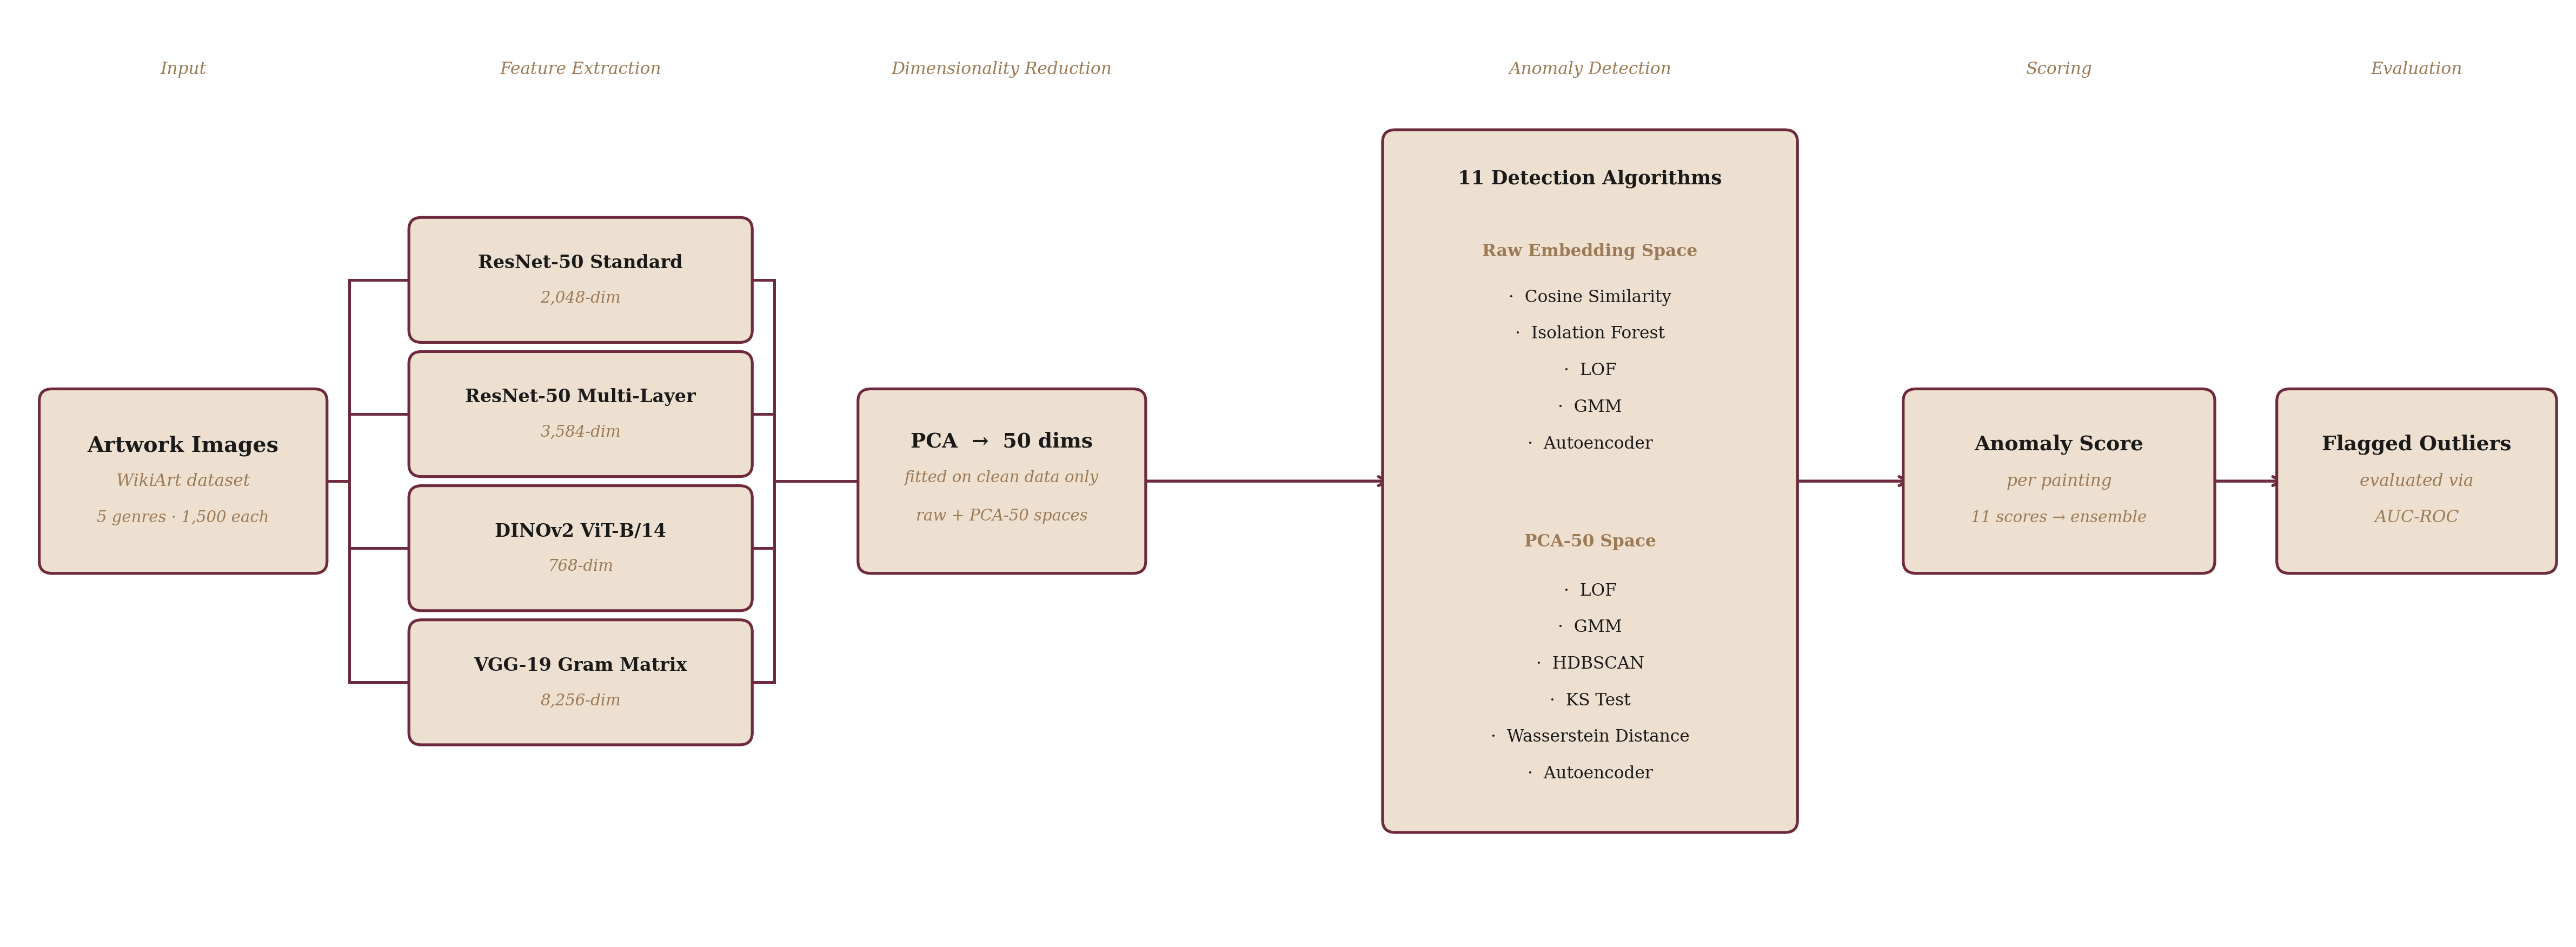
\includegraphics[width=\columnwidth]{figures/pipeline.png}
\caption{End-to-end pipeline. Each painting passes through four
pretrained visual representations. Embeddings are optionally projected to a 50-dim PCA subspace fitted on clean host-genre data. Eleven anomaly detectors score every painting, and AUC-ROC is computed against the injection labels.}
\label{fig:pipeline}
\end{figure}

\subsection{Problem formulation}

Let $G = \{x_1, \dots, x_N\}$ denote a set of $N$ paintings nominally belonging to a single genre. Each painting $x_i$ is mapped to an embedding vector $z_i = f_\theta(x_i) \in \mathbb{R}^d$ by a pretrained network $f_\theta$. The goal is a scoring function $s$ such that paintings that stylistically do not fit in $G$ receive higher scores than those that do. No labels are available during training. The only input is the distribution of embeddings from $G$ itself. This is an unsupervised one-class problem: the detector learns what the normal distribution looks like from the data alone, and anything that falls outside that pattern is scored as an anomaly.

\subsection{Dataset construction and genre selection}

Paintings are sourced from WikiArt~\cite{wikiart}. The dataset consists of 1{,}500 paintings from each of five canonical genres: Impressionism, Realism, Romanticism, Baroque, and Northern Renaissance. The five genres were chosen for both statistical and art-historical reasons. On the statistical side, 1{,}500 paintings per genre is large enough to train density and reconstruction models while still being manageable for the distance calculations that local outlier methods require. Keeping all genres the same size also avoids class imbalance when comparing detection performance across genres. On the art-historical side, the five genres were selected to cover a wide range of internal stylistic consistency. Impressionism is a stylistically tight movement defined by broken brushwork, outdoor light, and everyday subject matter. Realism overlaps with Impressionism in subject matter but uses more restrained brushwork and palette, which lets us test whether models can distinguish \emph{how something is painted} from \emph{what is depicted}. Romanticism is internally diverse, spanning landscape painting, history paintings, and emotionally charged portraiture, and tests how detectors handle high within-genre variation. Baroque is dramatic and compositionally dense, characterized by strong light and shadow, theatrical staging, and complex figure arrangements. Northern Renaissance is defined by precise draftsmanship, religious iconography, and fine detail. Together, Baroque and Northern Renaissance extend the dataset by several centuries beyond the nineteenth-century movements, so the evaluation is not limited to a narrow time window.

\subsection{Controlled anomaly injection}

Because real ground-truth stylistic anomalies are not available at scale, the study uses a controlled injection approach that produces clean binary labels while using real paintings throughout. For each host genre, 75 randomly sampled paintings from a set of anomaly genres replace 75 of the original 1{,}500, giving a 5\% contamination rate, which is standard in the anomaly-detection literature. Two injection regimes are evaluated. The standard regime draws anomalies from Cubism, Expressionism, and Abstract Expressionism, three movements that represent escalating degrees of structural disruption relative to representational nineteenth-century painting. These injections provide an upper bound on framework performance because the visual departure is severe and largely categorical. The hard regime injects paintings from Fauvism, Post-Impressionism, and Pointillism, movements that are stylistically and historically adjacent to Impressionism. Post-Impressionism literally descends from Impressionism, while Fauvism and Pointillism share its subject matter, palette range, and plein-air sensibility. Detection in the hard regime therefore tests whether models identify subtle stylistic departures rather than categorical ones, and approximates the practical scenario in which an analyst is screening a collection for outliers rather than for obvious misfilings.

\subsection{Visual representations}

Four deep visual representations are extracted per painting. The first three are semantic-content embeddings derived from networks trained on natural images. ResNet-50 \cite{resnet} pretrained on ImageNet provides a 2{,}048-dimensional vector from its global average-pooling output. A multi-layer ResNet-50 representation concatenates pooled activations from layers~2, 3, and~4 ($512 + 1{,}024 + 2{,}048 = 3{,}584$ dimensions), preserving mid-level texture information that would otherwise be discarded by the final pooling layer. DINOv2 ViT-B/14 \cite{dinov2} provides a 768-dimensional CLS-token embedding from a vision transformer trained self-supervised on a large image dataset, capturing global compositional structure through patch-wise self-attention. The fourth representation is qualitatively different. A flattened upper triangle of the Gram matrix of VGG-19 \cite{vgg} \texttt{conv2\_1} activations gives an 8{,}256-dimensional style embedding that encodes second-order channel co-occurrence statistics independently of depicted content. The Gram-matrix formulation is the established mathematical characterization of artistic style in the neural style-transfer literature \cite{gatys}. The four embeddings span the spectrum from pure semantic content (ResNet final pool, DINOv2) through mixed content and texture (multi-layer ResNet) to pure style texture (VGG Gram), which lets the study isolate the contribution of representation type to detection performance. All embeddings are $L_2$-normalized prior to detection.

\subsection{Dimensionality reduction}

Several detection algorithms are computationally or statistically infeasible in the raw embedding dimension. PCA projection to fifty components is applied as an optional preprocessing step. The projection is fitted only on the clean host-genre subset ($N=1{,}425$ per genre), so injected anomalies never influence the principal directions. Fifty components retain roughly 80--90\% of the variance across all four embedding types in the host distributions used here, and reduce the data to a regime in which HDBSCAN, full-covariance GMM, and distributional tests are tractable. The interaction between PCA and embedding family is itself an object of analysis and is reported in Section~\ref{sec:results}.

\subsection{Detection algorithms}

Eleven detection algorithms are evaluated, covering every major paradigm in unsupervised anomaly detection. On raw embeddings, the methods are cosine similarity to the genre mean (a distance baseline), Isolation Forest with 200 trees \cite{iforest}, Local Outlier Factor with $k=20$ neighbors and cosine distance \cite{lof}, a diagonal-covariance Gaussian Mixture Model with ten components, and a deep autoencoder trained for up to 150 epochs with mean-squared reconstruction error and early stopping on a held-out validation split of the normal data. On the PCA-50 space, the methods are LOF ($k=20$, Euclidean distance), GMM (ten components, full covariance), HDBSCAN (minimum cluster size 50, minimum samples 10)
\cite{hdbscan}, an autoencoder with smaller hidden dimensions, the
Kolmogorov--Smirnov test applied per dimension against a clean reference, and a sliced Wasserstein distance with 200 projections
\cite{swd}. Each method produces a real-valued anomaly score per
painting normalized to $[0,1]$. Hyperparameters are held fixed across genres to avoid per-genre tuning that would compromise generalization. Seeds are fixed at 42 throughout. End-to-end fine-tuning of the embedding networks and one-class deep classifiers such as Deep SVDD were tested but dropped, because they mix representation quality with task-specific optimization and make a fair comparison across embeddings impossible.

The choice of which methods to run in which space is not arbitrary. Cosine similarity and Isolation Forest are run on raw embeddings because their geometric assumptions degrade under PCA compression. Cosine relies on angular separation in the high-dimensional feature space, and Isolation Forest uses random axis-aligned splits that become uninformative after principal-component rotation. HDBSCAN, full-covariance GMM, KS, and sliced Wasserstein are restricted to PCA-50 because they break down in very high dimensions. HDBSCAN and KS are sensitive to the curse of dimensionality, and full-covariance GMM has $\mathcal{O}(d^2)$ parameters per component, which becomes intractable at the raw embedding sizes used here. LOF, diagonal-covariance GMM, and the autoencoder are evaluated in both spaces to isolate the effect of PCA reduction itself.

\subsection{Evaluation protocol and reproducibility}

Detection quality is measured by AUC-ROC against the binary injection labels. AUC-ROC is invariant to threshold choice and to the moderate class imbalance introduced by the 5\% injection rate, and is standard in the anomaly-detection literature. Each (embedding, method, genre, regime) cell yields a single AUC value. Aggregations report the mean and standard deviation across the five host genres.

The pipeline is exposed as Python scripts sharing a single \texttt{config.py} and parameterized by two environment variables, \texttt{EMBEDDINGS\_DIR} and \texttt{DATASET\_TYPE}. One end-to-end run, including embedding extraction, PCA fitting, all eleven detectors, and the summary notebook, is launched with a single shell command per configuration. Figures and tables are regenerated programmatically from the notebook \texttt{final\_results\_summary.ipynb}, and no number reported below is hand-edited. The implementation uses Python~3.11 with PyTorch, scikit-learn, and \texttt{hdbscan}. A pinned \texttt{requirements.txt} and a top-level \texttt{README.md} document the environment and reproduction steps.

\section{Results}
\label{sec:results}

\subsection{Aggregate performance}

Across all 440 AUC measurements, the autoencoder on raw embeddings is the strongest detector overall with mean AUC 0.872, followed by raw-space LOF at 0.756 and raw-space GMM at 0.755. The single best aggregate combination is multi-layer ResNet-50 paired with the raw autoencoder, reaching a mean AUC of $0.95 \pm 0.02$ on standard injection and $0.92 \pm 0.02$ on hard injection. The highest single cell is DINOv2 with the raw autoencoder on Baroque under standard injection, at 0.976. Fig.~\ref{fig:heatmap} shows the full embedding-by-method AUC matrix under both injection regimes. Tables~\ref{tab:embedding-rank} and~\ref{tab:method-rank} aggregate the measurements by embedding and by method respectively.

\begin{figure*}[t]
\centering
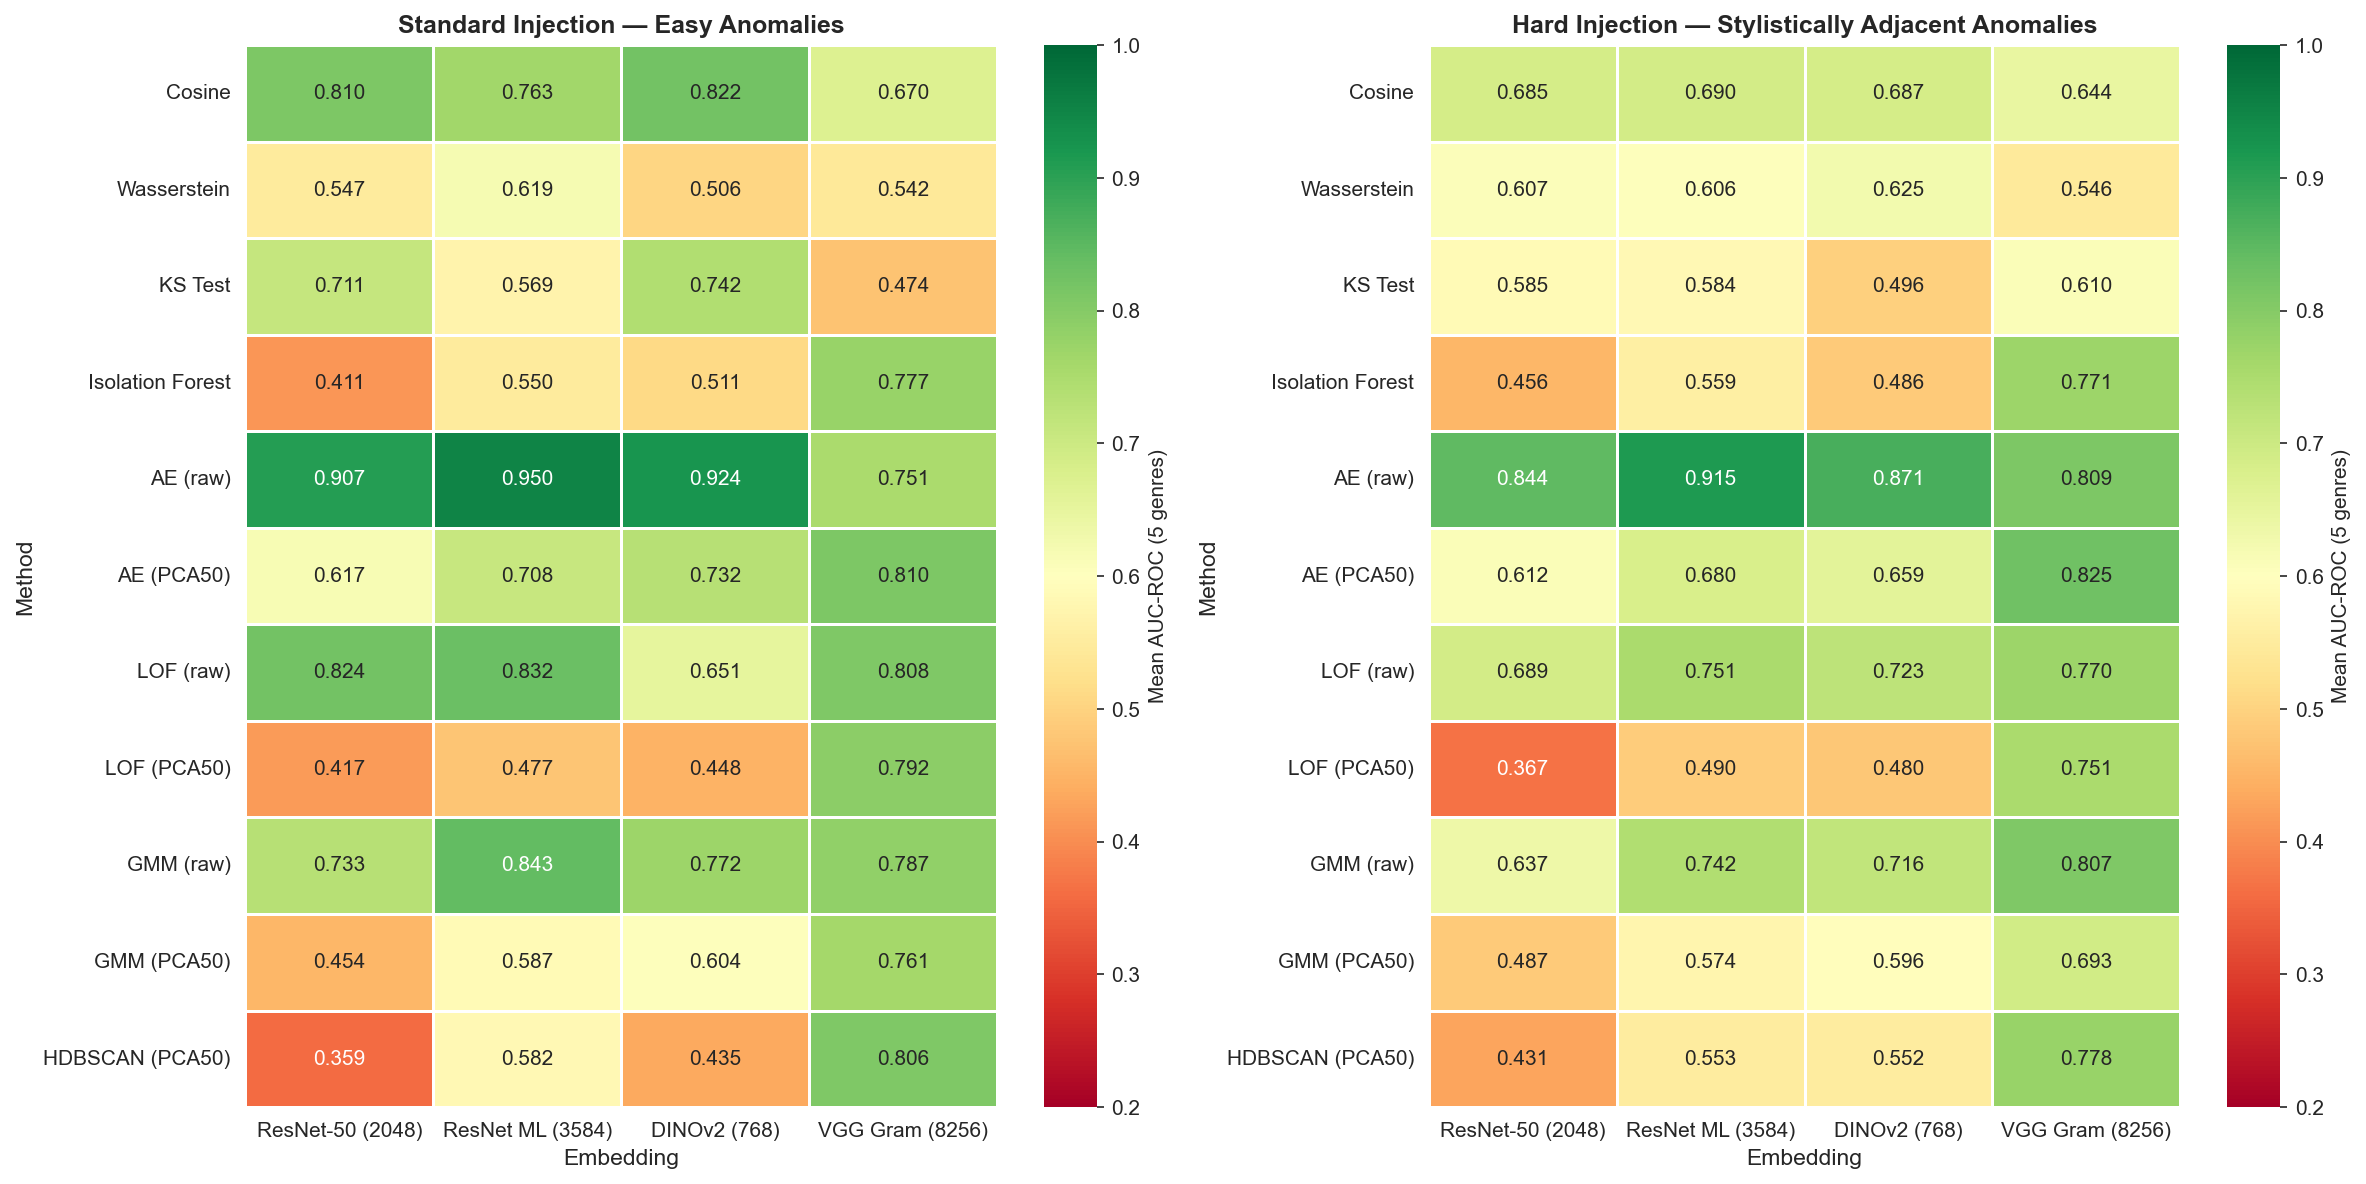
\includegraphics[width=\textwidth]{figures/heatmap.png}
\caption{Mean AUC-ROC across the five host genres for every
(embedding, method) pair. Left: standard injection. Right: hard injection. The optimal cell shifts between detectors and embedding spaces, motivating the analysis in Section~\ref{sec:rank-inversion}.}
\label{fig:heatmap}
\end{figure*}

\begin{table}[t]
\caption{Mean AUC-ROC by embedding ($n{=}110$ measurements per row).}
\label{tab:embedding-rank}
\centering
\begin{tabular}{lcc}
\toprule
\textbf{Embedding} & \textbf{Mean AUC} & \textbf{Std} \\
\midrule
VGG-19 Gram (8{,}256) & 0.727 & 0.114 \\
ResNet-50 multi-layer (3{,}584) & 0.665 & 0.147 \\
DINOv2 ViT-B/14 (768) & 0.638 & 0.158 \\
ResNet-50 standard (2{,}048) & 0.600 & 0.172 \\
\bottomrule
\end{tabular}
\end{table}

\begin{table}[t]
\caption{Mean AUC-ROC by detection method ($n{=}40$ measurements per row).}
\label{tab:method-rank}
\centering
\begin{tabular}{lc}
\toprule
\textbf{Method} & \textbf{Mean AUC} \\
\midrule
Autoencoder (raw)        & 0.872 \\
LOF (raw)                & 0.756 \\
GMM (raw)                & 0.755 \\
Cosine similarity        & 0.721 \\
Autoencoder (PCA-50)     & 0.705 \\
Kolmogorov--Smirnov      & 0.596 \\
GMM (PCA-50)             & 0.595 \\
Sliced Wasserstein       & 0.575 \\
Isolation Forest         & 0.565 \\
HDBSCAN (PCA-50)         & 0.562 \\
LOF (PCA-50)             & 0.528 \\
\bottomrule
\end{tabular}
\end{table}

\subsection{Method ranking inversion}
\label{sec:rank-inversion}

The most theoretically interesting finding is that detector rankings differ systematically between semantic and style embeddings (Fig.~\ref{fig:rank-inversion}). On semantic embeddings (ResNet standard, ResNet multi-layer, DINOv2), density-based and reconstruction-based detectors such as the autoencoder, LOF, and cosine similarity dominate. On VGG Gram features, isolation-based and distribution-based detectors (Isolation Forest, sliced Wasserstein, KS) move up the ranking. The reordering is stable across genres and across both injection regimes. Section~\ref{sec:analysis} explains the mechanism behind this pattern.

\begin{figure}[t]
\centering
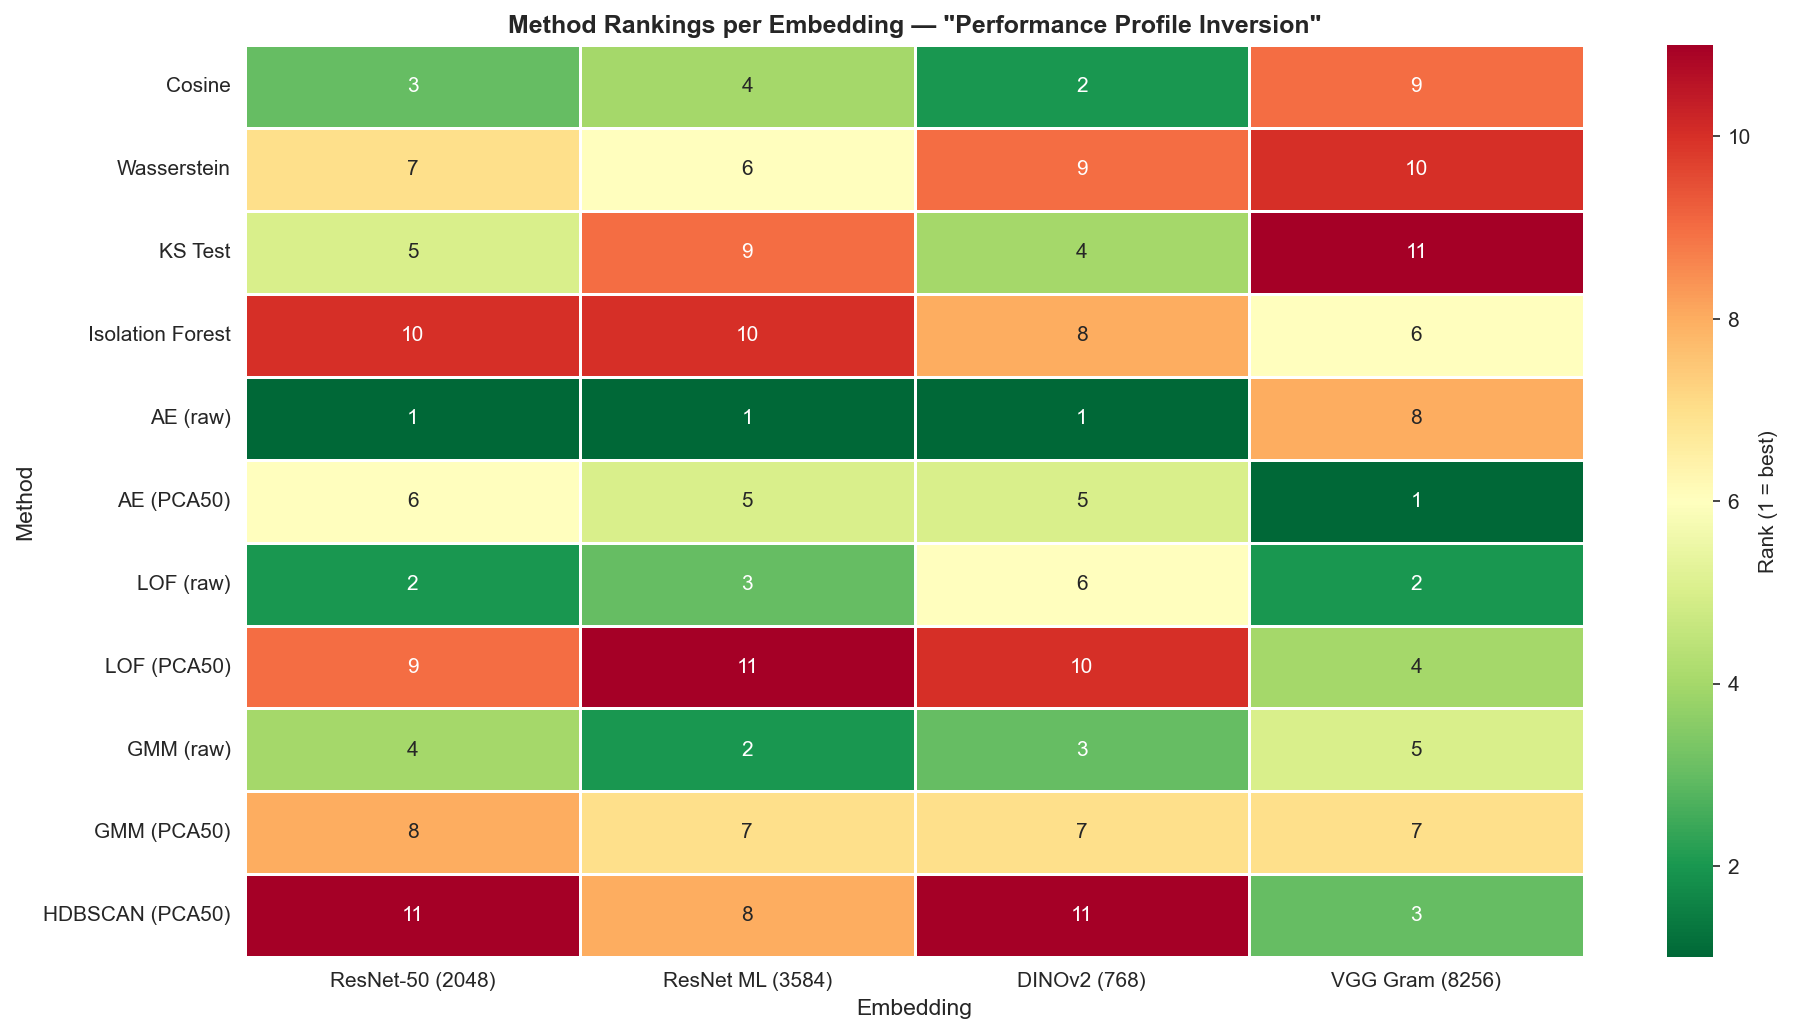
\includegraphics[width=\columnwidth]{figures/rank.png}
\caption{Method ranks per embedding (1~=~best). The reordering of
detectors between semantic embeddings and the VGG-19 Gram embedding is the central qualitative finding. Density- and reconstruction-based detectors win on semantic spaces, and isolation- and distribution-based detectors win on Gram space.}
\label{fig:rank-inversion}
\end{figure}

\subsection{Effect of PCA reduction}

Whether PCA helps or hurts depends entirely on the embedding family. For semantic embeddings (ResNet, DINOv2), PCA discards information that is relevant for detection. The autoencoder loses 0.07 to 0.10 AUC when moved from raw to PCA-50. For VGG Gram features, PCA actually helps: it concentrates redundant texture statistics into a smaller set of meaningful components, which makes distributional detectors more effective. Fig.~\ref{fig:pca-vs-raw} shows this contrast across all methods.

\begin{figure}[t]
\centering
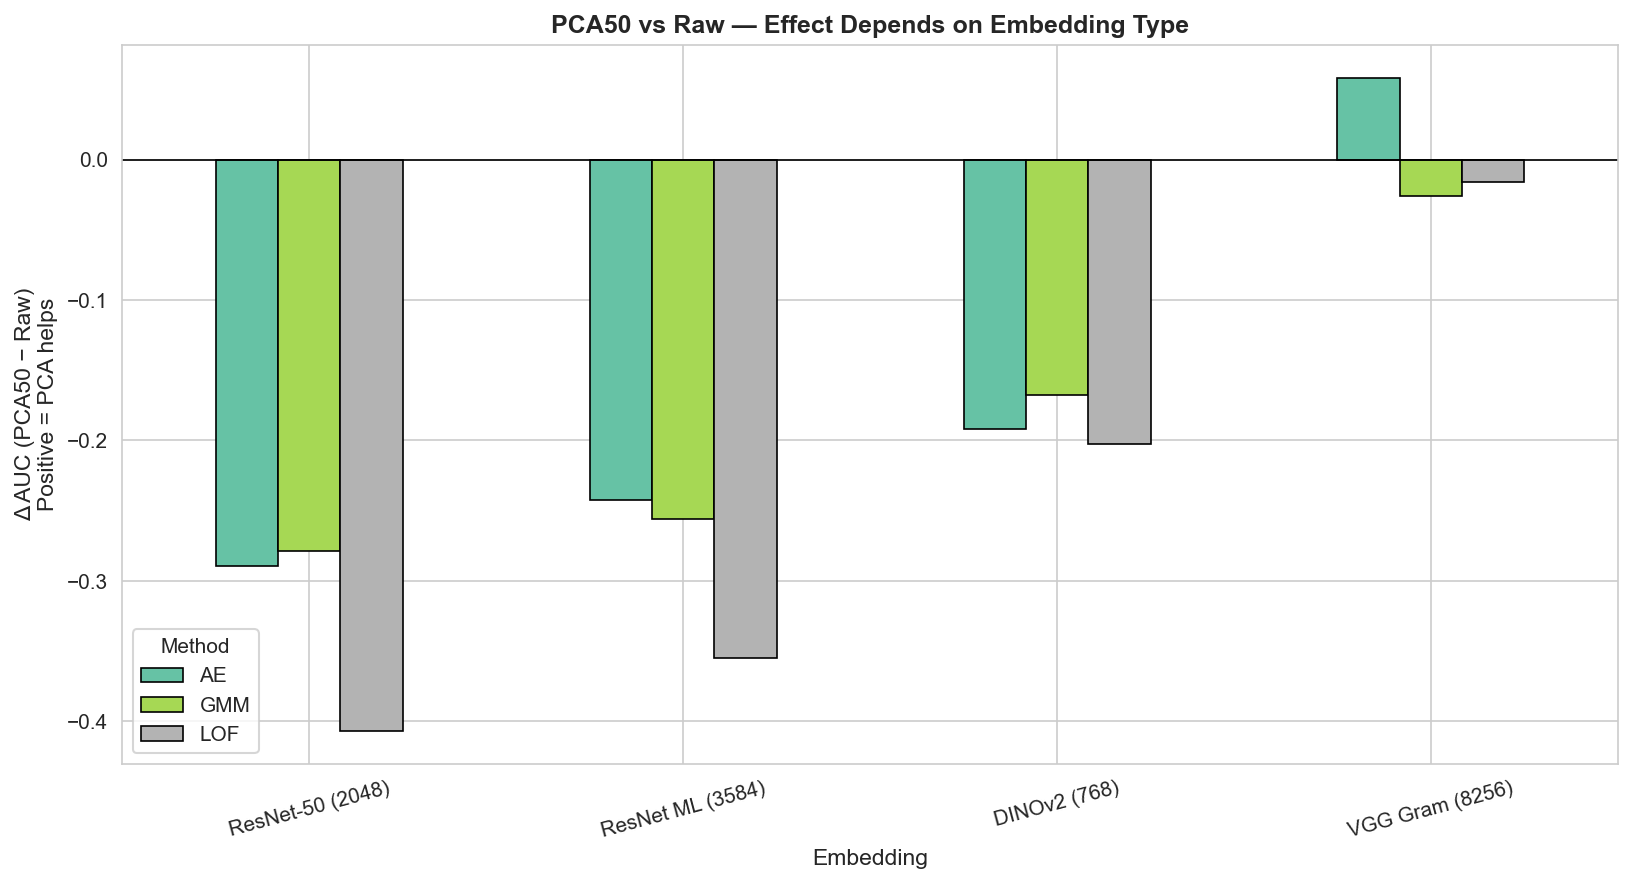
\includegraphics[width=\columnwidth]{figures/pca_vs_raw.png}
\caption{Mean AUC-ROC on raw embeddings vs.\ PCA-50 for each method.
PCA compression helps style-texture (VGG Gram) methods but hurts reconstruction-based methods on semantic embeddings.}
\label{fig:pca-vs-raw}
\end{figure}

\subsection{Effect of injection difficulty and genre}

Moving from standard to hard injection reduces mean AUC by 0.05 to 0.10 across embeddings (Fig.~\ref{fig:difficulty}). Detectors that rely on large distributional differences (Isolation Forest, Wasserstein) show the largest drops. The autoencoder loses the least, because it models the fine-grained structure of the host genre rather than relying on simple distance thresholds. The fact that the strongest combination still reaches AUC~0.92 on hard injection, where the injected paintings are historically and visually adjacent to the host genre, is the clearest evidence that the framework is responding to real stylistic signal.

\begin{figure}[t]
\centering
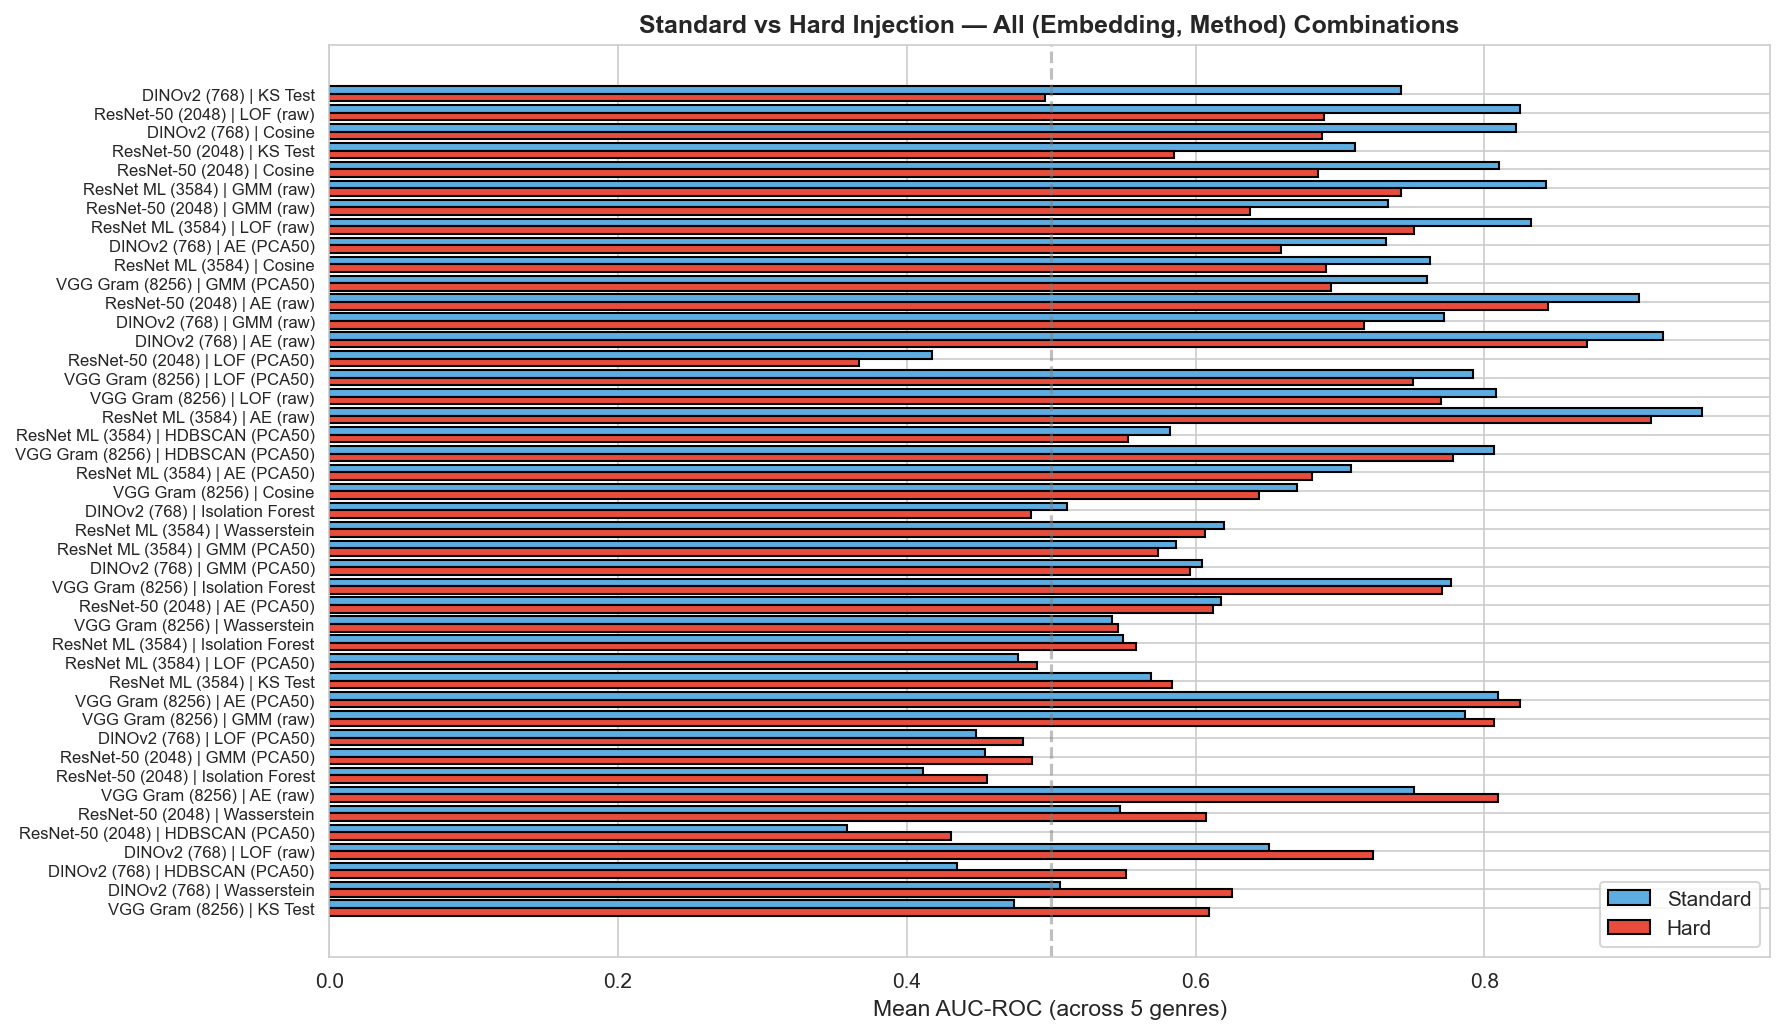
\includegraphics[width=\columnwidth]{figures/difficulty.png}
\caption{Mean AUC-ROC under standard injection vs.\ hard injection,
per embedding. Hard injection (Post-Impressionism, Fauvism, Pointillism) reduces performance across all embeddings, with the largest drop on VGG Gram.}
\label{fig:difficulty}
\end{figure}

Per-genre AUC varies substantially. Baroque and Northern Renaissance are the easiest genres, with peak AUC above 0.95. Romanticism is the hardest, with peak AUC roughly 0.05 to 0.08 lower than other genres for the same detector. Impressionism and Realism fall between these extremes. This ordering is stable across all embeddings and methods, which means it reflects real differences in how internally consistent each genre is, not a quirk of any single detector.

\section{Analysis and Validation}
\label{sec:analysis}

This section explains the results and validates the framework against external evidence. It covers four topics: a geometric explanation of the ranking inversion, an analysis of why VGG Gram leads on average while multi-layer ResNet leads at the top, per-genre and per-regime effects, and the qualitative expert review with concrete visual examples.

\subsection{Semantic vs. style geometry: why detector rankings invert}

The ranking inversion in Section~\ref{sec:rank-inversion} is the central scientific finding of this work and has a geometric explanation grounded in what each embedding represents.

Semantic embeddings mainly capture what is shown in a painting. When a Cubist painting is added into an Impressionist set, its features tend to fall in a part of the space where Cubist works are found and where Impressionist works are not. This makes the anomaly appear as a small, separate cluster or “pocket” in the feature space. An injected painting can be far from the main Impressionist group, but still close to other injected paintings from the same style.

Density-based methods like LOF and autoencoders are good at detecting this kind of structure. LOF compares the density of a point’s neighborhood to the density around nearby points, so it flags points that sit in unusually sparse regions. Autoencoders learn the structure of normal (host-genre) paintings, so injected paintings do not fit this learned pattern and end up with higher reconstruction error. Cosine similarity to the mean works in a similar way because injected styles tend to point in a different overall direction from the average of the host genre.

Style-texture embeddings, by contrast, encode how a painting is painted. A Cubist injection in an Impressionist collection is not just locally sparse. Its Gram statistics look different across the entire texture vocabulary. Cubist faceting produces channel patterns that are nearly orthogonal to the broken-brushwork patterns of Impressionism. The anomaly is no longer a small separated group inside a content-coherent space but a \emph{globally isolated cluster} of points whose statistical distribution is clearly different from the host genre. Detectors that operate on global distributional structure rather than local neighborhood density, therefore, move up the ranking. Isolation Forest exploits global isolation through random axis-aligned splits. The sliced Wasserstein distance and the Kolmogorov--Smirnov test compare empirical distributions and detect that the injected paintings violate the marginal statistics of the host genre.

The results show that different embeddings produce different anomaly structures, so detector performance depends strongly on the representation being used.

\subsection{Why VGG Gram wins on average but multi-layer ResNet wins at the top}

A pattern in Tables~\ref{tab:embedding-rank} and~\ref{tab:method-rank} that initially looks confusing is that VGG Gram has the highest aggregate mean AUC (0.727) while the single best embedding and method pair is multi-layer ResNet with the raw autoencoder. The two facts are not in tension. They answer different questions.

The aggregate ranking is dominated by \emph{consistency} across methods. VGG Gram performs respectably on a broad family of distributional and isolation-based detectors, so its mean across 110 measurements is high even though its peak is below the multi-layer ResNet peak. Multi-layer ResNet has higher variance instead. It achieves the strongest single result with the raw autoencoder but drops sharply on weaker detectors such as PCA-50 LOF. Its mean is therefore pulled down by the underperforming combinations even though the top combination is the best in the entire study.

This pattern has a practical implication. A deployment that can afford to identify and use the best embedding and method pair should prefer multi-layer ResNet with the raw autoencoder. A deployment that has to fix a single embedding and apply many detection methods to it, or that lacks the validation data to identify the best pair, should prefer VGG Gram because the latter is more forgiving of method choice.

\subsection{Per-genre effects: Baroque vs. Romanticism}

The systematic differences in AUC between genres are not artifacts of any single detector and align with art-historical characterizations of within-genre stylistic coherence. Baroque painting, despite its temporal breadth, is formally constrained by strong conventions of chiaroscuro, theatrical composition, and figural treatment. The within-genre embedding distribution is correspondingly tight, and even subtle injections land outside it. Northern Renaissance shares this formal constraint through religious iconography and high-precision draftsmanship.

Romanticism, by contrast, spans landscape, history painting, and emotional portraiture, with substantial stylistic variation among practitioners and across the movement's geography. Its within-genre embedding distribution is therefore broader, and any injection genre that shares emotional or atmospheric vocabulary with Romanticism overlaps with the host-genre cloud. Impressionism and Realism fall between these extremes. Each has clear conventions but exhibits considerable internal variety in subject and execution. The quantitative ordering of detection difficulty (Baroque and Northern Renaissance easier, Romanticism harder, Impressionism and Realism intermediate) is the same ordering an art historian would produce from formal-coherence intuitions alone, a point made explicitly during the expert review described below.

\subsection{Effect of injection difficulty}

The drop of 0.05 to 0.10 AUC when moving from standard to hard injection is informative about what the detectors are sensing. On standard injection the gap between Cubist or Abstract Expressionist injections and the representational host genre is so large that almost any detector with access to a usable representation reaches high AUC. The bottleneck is the representation, not the detector. On hard injection, where the injection genres are historically and visually adjacent to Impressionism, the gap is smaller and the detector's assumptions about how anomalies are distributed begin to matter. Detectors that rely on coarse distributional differences (Isolation Forest, Wasserstein) lose the most AUC. The autoencoder loses the least because its nonparametric capacity to model the normal structure of the host genre survives the increased difficulty.

The persistence of well-above-chance AUC under hard injection, including 0.92 for the strongest combination, is the strongest evidence that the framework is responsive to genuine stylistic signal rather than categorical surface differences. If the system only worked because Cubism is visually unlike Impressionism, performance would collapse when the injection comes from Post-Impressionism. It does not.

\subsection{Interpretability through reconstruction-error attribution}

Beyond the scalar anomaly score, the autoencoder produces a per-feature squared reconstruction error that can be mapped back to the painting. Fig.~\ref{fig:cam} shows these error heatmaps for Realism paintings flagged under hard injection. High-error regions cluster on the brushwork and palette areas that visually distinguish the injected genre from Realism: impasto and thick paint strokes in Post-Impressionist injections, broken color fields in Pointillist injections, and flattened chromatic regions in Fauvist injections. These are exactly the traits an art historian would name as the markers of those movements. Every anomaly score therefore comes with an explanation. An analyst can look at the error map to understand \emph{why} a painting was flagged, rather than accepting a number with no context.

\begin{figure}[t]
\centering
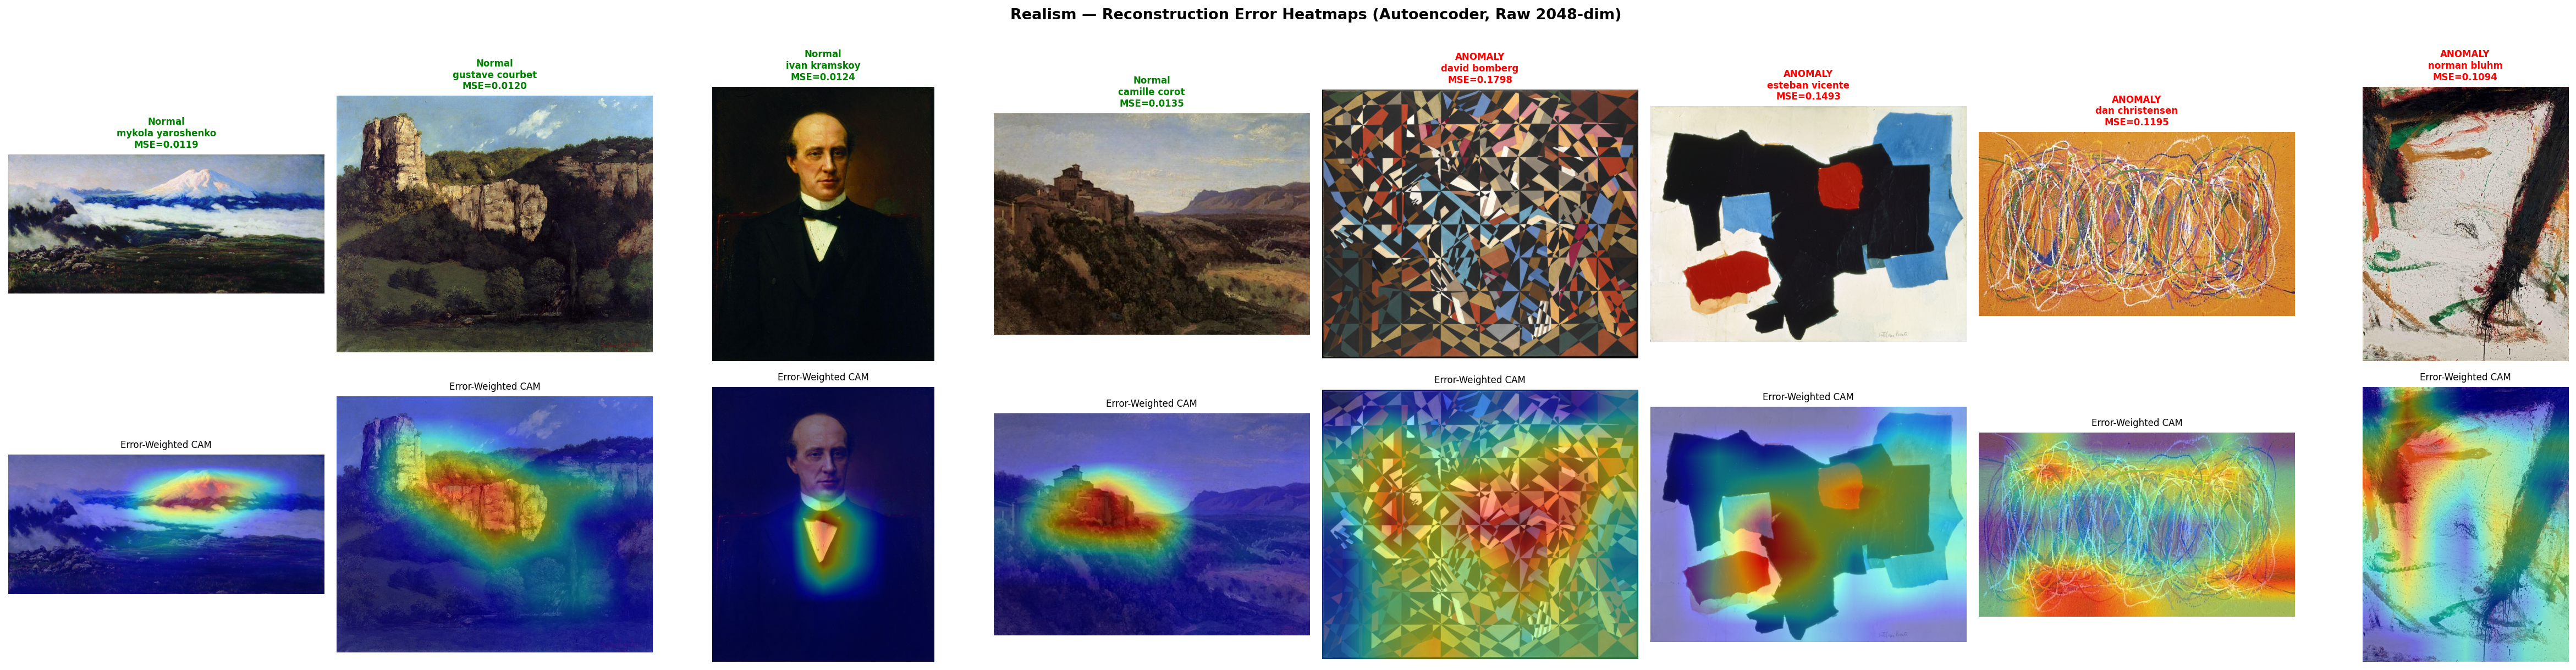
\includegraphics[width=\columnwidth]{figures/cam.png}
\caption{Autoencoder reconstruction-error heatmaps for Realism
paintings under hard injection. The highest-error regions align with the stylistically distinctive traits of the injected genre, making the anomaly signal directly interpretable.}
\label{fig:cam}
\end{figure}

\subsection{Expert validation}

A qualitative review of the model outputs was conducted by Prof.\ Emma Chookaszian, who teaches the \emph{Introduction to Art} course at the American University of Armenia. Her observations engage directly with both the strengths and the limitations of the framework. Four observations are summarized here for their methodological implications.

First, several works flagged most strongly by semantic embeddings shared distinctive depicted content (recurring still-life arrangements, specific compositional templates) rather than distinctive brushwork. This aligns with the fact that ImageNet-pretrained networks are primarily designed for object recognition, so they capture “what” is shown in an image as much as “how” it is visually rendered. In practice, this suggests that systems should combine semantic and Gram-based representations, since they capture different but complementary aspects of visual information, as discussed in Section~\ref{sec:rank-inversion}.

Second, art-historical analysis is more detailed than the genre labels used in WikiArt. Artists change styles over time, artistic movements contain different sub-traditions, and some historically important sub-genres, such as Baroque still life, may appear rarely in the dataset without actually being anomalies. Since the current framework models each genre as a single group, it can assign high anomaly scores to works that are historically valid but less common within the dataset. This does not mean the framework is incorrect, but rather that its results should be interpreted together with art-historical context.

Third, what appears most often in a dataset is not necessarily what best represents an artistic movement. WikiArt and museum-based collections reflect curatorial choices and dataset availability rather than the true historical distribution of artistic styles. Important or movement-defining works may appear less frequently than more repetitive or derivative ones. As a result, a purely statistical system may learn the “average” style of the dataset instead of the most historically significant one. This is an important limitation and shows why the framework’s outputs should not be treated as final art-historical judgments without expert interpretation.

Fourth, detection performance was strongest on the genres the professor described as the most formally controlled (Baroque, Northern Renaissance) and weakest on the most internally heterogeneous (Romanticism). This correspondence between AUC and art-historical assessments of stylistic coherence provides external validation of the framework, since the expert's qualitative ordering was elicited independently of the quantitative results. The review also identified that several flagged paintings were misclassified non-painting media (sculpture photographs, fresco reproductions), which indicates that medium filtering is a necessary preprocessing step for any deployment beyond the curated experimental setup.

Fig.~\ref{fig:gallery} shows the top-scored anomalous paintings for Northern Renaissance under standard injection. The flagged works are visually distinct from the genre: they lack the precise draftsmanship, religious iconography, and fine-detail character that define Northern Renaissance, and the professor confirmed these observations independently during the review.

\begin{figure}[t]
\centering
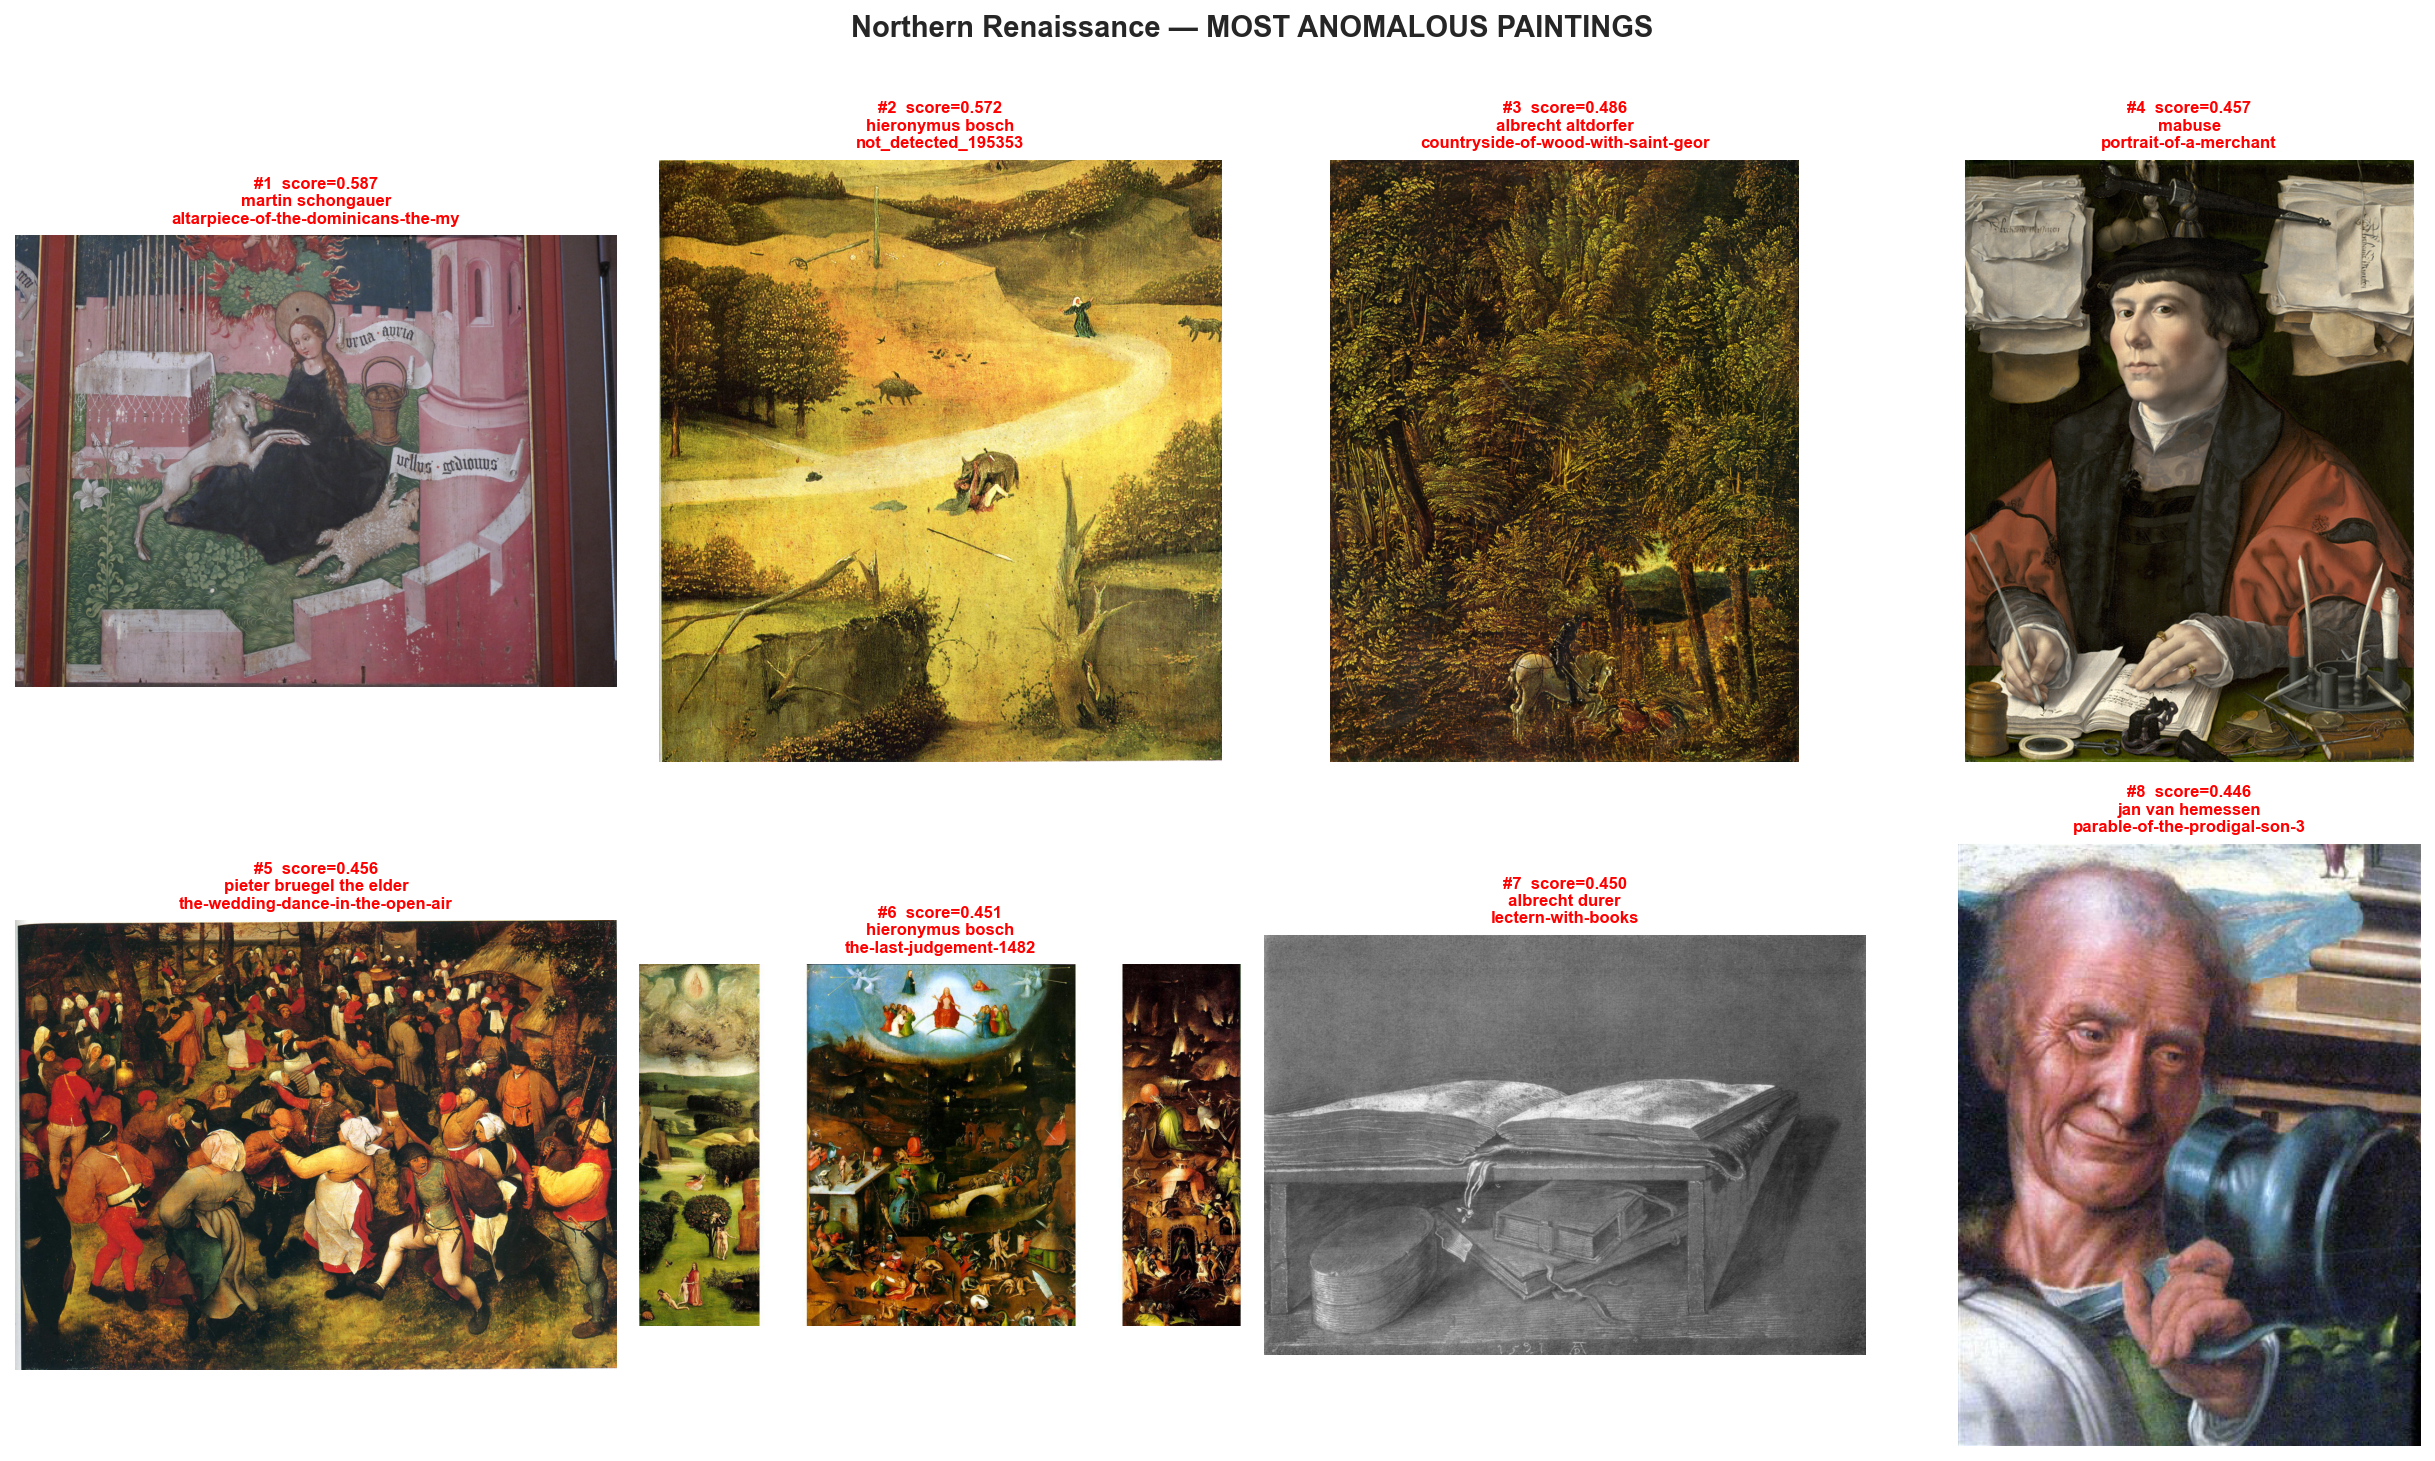
\includegraphics[width=\columnwidth]{figures/gallery.png}
\caption{Top anomalous paintings flagged by the autoencoder for
Northern Renaissance under standard injection. All shown works were injected from a different genre and differ visibly from the precision-draftsmanship character of the host genre.}
\label{fig:gallery}
\end{figure}

\subsection{Validation against project objectives}

The original proposal specified three objectives: benchmark multiple deep representations in a single evaluation setup, analyze how well normal and anomalous paintings separate in embedding space, and provide interpretable visualizations of the anomaly signal. The first is met by the 440-cell evaluation in Tables~\ref{tab:embedding-rank} and~\ref{tab:method-rank}. The second is addressed by the density-based detectors (LOF, GMM, Cosine) and supported by the correspondence between AUC and the expert-described internal coherence of each genre. The third is addressed by the reconstruction-error attribution in Fig.~\ref{fig:cam}. Every reported pipeline achieves AUC strictly greater than the 0.5 random baseline on at least one genre.

\section{Limitations and Practical Considerations}
\label{sec:discussion_limitation}

Several limitations bound the interpretation and generalizability of the findings. Each is stated explicitly because the framework is intended for use by non-machine-learning specialists who should understand its scope.

\textbf{Synthetic evaluation protocol.} The injection methodology
provides clean binary ground truth, but the anomalies studied here are drawn from movements with no historical connection to the host genre. Attested historical anomalies, such as misattributed works discovered after archival research, may have subtler or composite stylistic signatures that differ from injected paintings. Validation on real curatorial decisions or documented attribution revisions remains future work.

\textbf{Label noise in the source data.} WikiArt genre labels are
crowd-sourced and have not been verified against any academic authority. The pipeline cannot distinguish between a true stylistic outlier and a painting that was correctly executed in the genre but incorrectly tagged. The expert review surfaced both mislabeled non-painting media and likely genre-tag errors among the highest-scoring works, which confirms that label noise affects both the normal training distribution and the interpretation of high scores.

\textbf{Domain mismatch in pretrained representations.} All four
embeddings come from models trained on natural photographs rather than paintings. The gap between photographs and painted surfaces is not trivial. Brushwork texture, pigment granularity, and craquelure introduce visual patterns absent from photographic training data. The VGG-19 Gram embedding is the most affected because it explicitly encodes low-level texture co-occurrences, which carry different statistical regularities on paint than on photographs. Fine-tuning on a large set of paintings would partially close this gap and is identified below as a future direction.

\textbf{Flat genre norm.} The framework treats each genre as a
single distribution. Art-historical practice recognizes that movement-defining masterworks and derivative contemporaries should not carry equal weight in defining the norm, that movements contain sub-traditions, and that artists evolve across periods. A flat distribution misrepresents this structure and can flag canonical but rare sub-genres as outliers.

\textbf{Geographic and temporal scope.} The five evaluated genres
are Western European movements spanning the fifteenth through nineteenth centuries. The framework has not been evaluated on non-Western traditions, contemporary or abstract art, or decorative arts and craft media. Generalization across these domains is not established.

\textbf{Scope of the system as deployed.} This framework is not an
authentication or forgery-detection system. Authentication depends on provenance documentation, material analysis, pigment dating, and historical records, none of which a visual model can replace. The right way to think about this system is as a quantitative first filter. It ranks paintings in a large digital collection by how unusual they look, so human experts can direct their attention to the most suspicious cases rather than reviewing everything from scratch. The final judgment is always human.

\section{Conclusion}
\label{sec:conclusion}

This paper compared four deep visual embeddings and eleven anomaly-detection algorithms on a 7{,}500-painting WikiArt subset under two injection regimes. The main contributions are: a 440-cell comparison of the full embedding and detector design space (Figs.~\ref{fig:heatmap}--\ref{fig:difficulty}), a documented and geometrically explained ranking inversion between semantic and style-texture representations, a fully reproducible end-to-end pipeline, and an expert art-historian review with concrete visual examples (Figs.~\ref{fig:cam}--\ref{fig:gallery}). Each research question is answered below.

\textbf{RQ1 (best embedding and method combination).} Across 440
measurements, multi-layer ResNet-50 with a deep autoencoder on raw embeddings was the strongest combination, achieving a mean AUC-ROC of 0.95 on standard injection and 0.92 on hard injection. No single pipeline dominates universally, because semantic and style embeddings respond to different detector families. The practical recommendation is therefore conditional. Prefer multi-layer ResNet with the raw autoencoder when the best pair can be identified and tuned, and prefer VGG Gram when robustness to method choice is more important than peak performance.

\textbf{RQ2 (effect of PCA-50 reduction).} PCA reduction is not
uniformly beneficial, as shown in Fig.~\ref{fig:pca-vs-raw}. It degrades semantic embeddings by discarding variance that matters for detection, with the autoencoder losing 0.07 to 0.10 AUC on ResNet and DINOv2 when moved from raw to PCA-50. It improves style-texture embeddings by concentrating redundant Gram statistics into a smaller number of high-variance components. The projection should be applied selectively based on the embedding's variance structure, not as a default step.

\textbf{RQ3 (localization of the anomaly signal).}
Reconstruction-error attribution, shown in Fig.~\ref{fig:cam} for Realism, localizes anomalies to stylistically distinctive regions: impasto in Post-Impressionist works, broken color in Pointillist injections, and flat chromatic regions in Fauvist paintings. These regions match what an art historian would identify as the diagnostic markers of those movements. Every scalar anomaly score therefore comes with a spatial explanation that an analyst can inspect directly.

As shown in Section~\ref{sec:rank-inversion}, different types of embeddings work best with different anomaly detectors. Methods that perform well on semantic embeddings are not always the strongest on style-texture embeddings. Combining both content-based and style-based representations therefore provides curators, attribution researchers, and art historians with a more reliable and balanced analysis tool.

Four directions for future work come out of the expert review and the limitations above. First, fine-tuning the backbone networks on a large set of paintings, ideally using self-supervised objectives similar to DINOv2, would reduce the domain gap between natural photographs and historical paint surfaces. Second, replacing the flat genre distribution with a model that recognizes sub-traditions and tracks how individual artists evolve would reduce false positives on canonical but numerically rare works. Third, testing the framework against real documented misattributions from museum or gallery collections would move the evaluation beyond synthetic injection and toward practical grounding. Fourth, adding gradient-based saliency methods such as Grad-CAM~\cite{gradcam} alongside the autoencoder attribution would produce spatial explanations directly on the painting image, which are easier for art historians to read than abstract error maps in feature space.

This framework is not a replacement for art-historical expertise. It is a tool for handling the scale at which manual review is no longer practical. The system flags which paintings in a large digital collection look stylistically out of place. The curator or art historian then decides what to do with that information. This work makes that kind of systematic screening quantitative and reproducible.

\section*{Acknowledgments}

The author thanks Prof.\ Emma Chookaszian for her expert art-historical perspective and qualitative validation of the framework's outputs, and Prof.\ Narine Sarvazyan for her guidance on the structure and presentation of this work.

\bibliographystyle{IEEEtran}
\bibliography{references}

\end{document}

\end{document}
